% Replace "([a-z$,])\n(\s*)([$\(a-z])" with "$1 $3"
% Replace "\.\s([a-z])" with ". \n$1"
% Define document class & import showyourwork
\documentclass[modern]{aastex631}

% Packages
\usepackage{xifthen}
\usepackage{array}
\usepackage{upgreek}
\usepackage[bbgreekl]{mathbbol}
\usepackage{afterpage}
\usepackage[bb=boondox]{mathalpha}
\usepackage{tipa}
\usepackage{booktabs}


% Shorthand for this paper
\newcommand{\starry}{\textsf{starry}\xspace}
\newcommand{\Python}{\textsf{Python}\xspace}
\newcommand{\cpp}{\textsf{C}++\xspace}
\newcommand{\bvec}[1]{{\ensuremath{\mathbf{#1}}}}
\newcommand{\xxx}[1]{{\color{red}#1}}
\DeclarePairedDelimiter\floor{\lfloor}{\rfloor}
\DeclarePairedDelimiter\ceil{\lceil}{\rceil}
\newcommand{\imag}{{\ensuremath{\mathbb{i}}}}
\renewcommand{\quad}{\hskip 0.33em}
\newcommand{\quadquad}{\quad\quad\quad\quad}

\newcommand{\R}{\bvec{R}}
\newcommand{\AOne}{\bvec{A_1}}
\newcommand{\alm}{\bvec{a}}
\newcommand{\x}{\bvec{x}}
\newcommand{\D}{D}
\newcommand{\Doppler}{\bvec{D}}
\newcommand{\Surf}{\mathcal{S}}
\newcommand{\Curve}{\mathcal{C}}
\newcommand{\Dargs}{\bvec{d}}
\newcommand{\lmax}{\ensuremath{l_\mathrm{max}}}
\newcommand{\spot}{\texttt{SPOT}\xspace}
\newcommand{\vogtstar}{\texttt{VOGTSTAR}\xspace}
\newcommand{\kT}{\boldsymbol{\kappa}^\top}
\newcommand{\rhoT}{\boldsymbol{\rho}^\top}
\newcommand{\ylmbasis}{\boldsymbol{\psi}^\top}
\newcommand{\pbasis}{\boldsymbol{\phi}^\top}
\newcommand{\pbasisn}{\ensuremath{\phi_n}}
\newcommand{\almt}{\ensuremath{\bvec{a}}}
\newcommand{\lnlam}{\mbox{\textipa{\textcrlambda}}}

% Begin!
\begin{document}

% Title
\title{A Closed-Form Solution to the Doppler Imaging Problem}

% Author list
\author[0000-0002-0296-3826]{Rodrigo Luger}
\email{rluger@flatironinstitute.org}
\affil{Center~for~Computational~Astrophysics, Flatiron~Institute, New~York, NY}
%
\author{Megan Bedell}
\affil{Center~for~Computational~Astrophysics, Flatiron~Institute, New~York, NY}
%
\author{Daniel Foreman-Mackey}
\affil{Center~for~Computational~Astrophysics, Flatiron~Institute, New~York, NY}
%
\author{David W. Hogg}
\affil{Center~for~Computational~Astrophysics, Flatiron~Institute, New~York, NY}

\begin{abstract}
    We derive a closed form, analytic solution to the problem of Doppler imaging of stellar surfaces in the limit of negligible differential rotation and convective blueshift.
    The model for the observed spectrum is linear in the coefficients of the spherical harmonic expansion of the specific intensity distribution on the surface and, in certain limits, the posterior over surface maps has a closed form, analytic solution that is computationally trivial to evaluate.
    The model is also linear in the local (rest frame) stellar spectrum, which may itself be spatially variable.
    This allows one to perform Doppler imaging without knowledge of the local stellar spectrum and therefore works on blended lines or regions of the spectrum where line formation mechanisms are not well understood.
    Finally, the model is fast, differentiable, and allows one to calculate uncertainties on the inferred surface map.
\end{abstract}

% Main body
\section{Introduction}
The paper is organized as follows: in \S\ref{sec:the_problem}~and~\S\ref{sec:the_solution} we introduce the math behind the Doppler imaging problem and derive a closed form expression for the model. 
In \S\ref{sec:linear},~\S\ref{sec:inverse},~and~\S\ref{sec:bellswhistles} we demonstrate how to re-express the model as a linear operation on the input spectrum and stellar map and derive closed form expressions for the two conditioned on the data and priors.
In \S\ref{sec:spotstar} we apply our techniques to a mock problem. 
We further discuss and summarize our results in \S\ref{sec:discussion}~and~\S\ref{sec:conclusions}. 
Finally, auxiliary derivations are presented in the Appendix.

\section{The problem}
\label{sec:the_problem}
%
Let $I(\lnlam, \x, t, \Dargs)$ be the specific intensity observed at log wavelength $\lnlam \equiv \ln\frac{\lambda}{\lambda_\mathrm{r}}$ and at sky-projected Cartesian position $\x = (x, y, z)$ on the surface of the star at time $t$, where $\Dargs$ is a set of arbitrary parameters of the Doppler field and $\lambda_\mathrm{r}$ is a reference wavelength.
We may express this intensity as
%
\begin{align}
    \label{eq:the_problem:Ixi}
    I(\lnlam, \x, t, \Dargs) & =
    I\Big(\lnlam_0 + \D(\x, \Dargs), \x, t\Big)
\end{align}
%
where $\lnlam_0$ is the log wavelength in the rest frame and $\D$ is the Doppler shift in log wavelength space:
%
\begin{align}
    \label{eq:the_problem:D}
    \D(\x, \Dargs)
     & =
    \frac{1}{2}\ln\left(
    \frac{1 + \beta(\x, \Dargs)}{1 - \beta(\x,
            \Dargs)}
    \right)
\end{align}
%
where $\beta = v(\x, \Dargs) / c$ is the ratio of the radial velocity at a point on the surface of the star to the speed of light.
In keeping with the literature, we take positive values of $v$ (and $\D$) to mean redshifts.

A common approach to computing the Doppler-shifted spectrum is to evaluate the spectrum at the rest frame wavelength $\lnlam_0$ and interpolate back to the grid in $\lnlam$. 
This is practical when computing the spectrum at a single \emph{point} on the surface, but not ideal when one is interested in the \emph{integral} over the visible surface of the star $\Surf$, which is typically all we can observe:
%
\begin{align}
    \label{eq:the_problem:F}
    F(\lnlam, t, \Dargs)
     & \equiv
    \iint\limits_{\Surf(\x)}
    I(\lnlam, \x, t, \Dargs)
    \mathrm{d}{\Surf(\x)}
    \quad ,
\end{align}
%
The difficulty in solving Equation~(\ref{eq:the_problem:F}) stems from the fact that $I(\lnlam, \x, t, \Dargs)$ is difficult to write down in closed form, given the nonlinearity of the Doppler shift.
The standard approach to solving this integral is therefore to discretize the surface of the star with a fine grid, evaluate the Doppler-shifted spectrum in each cell, and sum over the spatial axes to approximate the integral. 
Depending on the resolution of the grid, this is either numerically inaccurate or computationally inefficient (and often both).

\section{The Solution}
\label{sec:the_solution}

\subsection{Doppler Deconvolution}

The observed spectrum is a complex function of spatial, spectral, temporal, and velocity terms. 
The goal in this section is to deconvolve each of these terms to make solving the integral in Equation~(\ref{eq:the_problem:F}) easier.
%
The first thing we will do is to express Equation~(\ref{eq:the_problem:Ixi})
as a convolution:
%
\begin{align}
    \label{eq:deconv:convolution}
    I(\lnlam, \x, t, \Dargs) & =
    I(\lnlam_0, \x, t)
    *
    \delta\big(\lnlam_0 + \D(\x, \Dargs)\big)
\end{align}
%
where $\delta$ is the Dirac delta function and $*$ denotes the linear convolution operator, defined for two arbitrary functions $g$ and $h$ as the integral
%
\begin{align}
    \label{eq:deconv:convolution_def}
    (g * h)(t) \equiv \int_{-\infty}^\infty g(\tau) h(t - \tau) d\tau
\end{align}
%
for some independent coordinate $t$ and dummy parameter $\tau$.
%
The convolution of $I(\lnlam_0)$ with a delta function has the effect of shifting the spectrum by an amount $\D$, returning a function of the shifted (observed) log wavelength, $\lnlam = \lnlam_0 + \D$.

Next, we expand the spatial dependence of the specific intensity at the rest frame wavelength in terms of spherical harmonics on the unit disk:
%
\begin{align}
    \label{eq:deconv:Ixi0}
    I(\lnlam_0, \x, t)
     & =
    \sum_{l=0}^{l_\mathrm{max}}\sum_{m=-l}^{l} a_{lm}(\lnlam_0, t) Y_{lm}(\x)
    \quad ,
\end{align}
%
where $Y_{lm}(\x)$ is a spherical harmonic on the projected disk and $a_{lm}(\lnlam_0, t)$ is the corresponding spherical harmonic coefficient at log wavelength in the rest frame $\lnlam_0$ and time $t$. 
For convenience, we may write this equation in vector form:
%
\begin{align}
    \label{eq:deconv:Ivec}
    I(\lnlam_0, \x, t) & =
    \ylmbasis(\x) \,
    \alm(\lnlam_0, t)
    \quad ,
\end{align}
%
where
%
\begin{align}
    \label{eq:deconv:alm}
    \alm(\lnlam_0, t) \equiv
    \Big(
    a_{0,0}(\lnlam_0, t) \quad 
    a_{1,-1}(\lnlam_0, t) \quad 
    a_{1,0}(\lnlam_0, t) \quad 
    a_{1,1}(\lnlam_0, t) \quad
    ...
    \Big)^\top
\end{align}
%
is the vector of $N = (l_\mathrm{max} + 1)^2$ spherical harmonic coefficients and
%
\begin{align}
    \label{eq:deconv:ylmbasis}
    \ylmbasis(\x) \equiv
    \Big(
    Y_{0,0}(\x) \quad 
    Y_{1,-1}(\x) \quad 
    Y_{1,0}(\x) \quad 
    Y_{1,1}(\x) \quad
    ...
    \Big)
\end{align}
%
is the corresponding vector of $N$ spherical harmonics. 
We may further decompose our expression by linearizing the time dependence of the spherical harmonic coefficients:
%
\begin{align}
    \label{eq:deconv:R}
    \alm(\lnlam_0, t) = \R(t) \, \azero(\lnlam_0)
    \quad ,
\end{align}
%
where $\azero(\lnlam_0) = \bvec{a}(\lnlam_0, t=t_0)$ for some reference time $t_0$.
For rigid body rotation, the result is exact and $\R(t)$ is the $(N \times N)$ Wigner rotation matrix for real spherical harmonics
\citep[e.g.][]{AlvarezCollado1989}, which is implicitly a function of the inclination, obliquity, and rotation period of the star.
%In the case that other processes such as differential rotation or spot 
%evolution are significant
%over the course of an observation, Equation~(\ref{eq:deconv:R}) can be
%made to hold approximately for some effective rotation matrix 
%$\R(t)$; we discuss this later.

The equation for the specific intensity in the rest frame now reads
%
\begin{align}
    \label{eq:deconv:Ivecfull}
    I(\lnlam_0, \x, t) & =
    \ylmbasis(\x)
    \,
    \R(t)
    \,
    \azero(\lnlam_0)
    \quad ,
\end{align}
%
where it is clear that we have fully separated the spatial, temporal, and spectral terms. 
Inserting this into Equation~(\ref{eq:deconv:convolution})
and integrating over the visible portion of the star, we arrive at the expression for the observed spectrum:
%
%
\begin{align}
    \label{eq:deconv:F2d}
    F(\lnlam, t, \Dargs) & =
    \iint\limits_{\Surf(\x)}
    \ylmbasis(\x)
    \,
    \R(t)
    \,
    \alm(\lnlam_0)
    * \delta\big(\lnlam_0 + \D(\x, \Dargs)\big)
    \mathrm{d}\Surf(\x)
    \nonumber                \\[0.5em]
                         & =
    \iint\limits_{\Surf(\x)}
    \ylmbasis(\x)
    \delta\big(\lnlam_0 + \D(\x, \Dargs)\big)
    \mathrm{d}\Surf(\x)
    \,
    \R(t)
    \,
    *
    \,
    \azero(\lnlam_0)
    \quad ,
\end{align}
%
%
where we made use of the commutativity of the convolution operator and the fact that the integral is taken only over the spatial dimensions.
Note, importantly, that the convolution operation above is implicitly a vector operation---i.e., the convolution is taken for each spherical harmonic term individually and then summed over all terms.

Finally, we can simplify Equation~(\ref{eq:deconv:F2d}) by noting that the delta function in the integrand allows us to reduce the double integral to a line integral:
%
\begin{align}
    \label{eq:deconv:kT}
    \iint\limits_{\Surf(\x)}
    \ylmbasis(\x)
    \delta\big(\lnlam_0 + \D(\x, \Dargs)\big)
    \mathrm{d}\Surf(\x)
    \, \,
     & =
    \int\limits_{\Curve(\lnlam, \x, \Dargs)}
    \hspace*{-0.6em}\ylmbasis(\x)
    \mathrm{d}\Curve(\lnlam, \x, \Dargs)
    \nonumber                     \\[0.5em]
     & \equiv \kT(\lnlam, \Dargs)
    \quad.
\end{align}
%
where the path $\Curve(\lnlam, \x, \Dargs)$ corresponds to the set of all points on the visible disk where $\lnlam_0 + \D(\x, \Dargs) = 0$.
%
We thus have
%
\begin{align}
    \label{eq:deconv:F}
    F(\lnlam, t, \Dargs)
     & =
    \kT(\lnlam, \Dargs) \, \R(t)
    *
    \azero(\lnlam_0)
    \quad.
\end{align}
%
Equation~(\ref{eq:deconv:F}) is the deconvolution of the observed spectrum into velocity terms, temporal terms, and spectral/spatial terms, respectively. 
In the next section, we will discuss how to efficiently solve the line integral in Equation~(\ref{eq:deconv:kT}).

\subsection{Computing the kernel $\kT$}
\label{sec:kT}
%
In the case that the star's rotation is rigid (i.e., differential rotation is negligible) and other effects such as convective blueshift may be ignored, the radial velocity at any point on the surface is simply proportional to the distance to the axis of rotation. 
Without loss of generality, if we assume the axis of rotation lies along the $y-z$ plane, we have
%
\begin{align}
    \label{eq:kT:beta}
    \beta(\x, \Dargs) = \frac{\omega \sin i \, x}{c}
\end{align}
%
and
%
\begin{align}
    \label{eq:kT:D}
    \D(\x, \Dargs) & =
    \frac{1}{2}\ln\left(
    \dfrac{1 + \dfrac{\omega \sin i \, x}{c}}
    {1 - \dfrac{\omega \sin i \, x}{c}}
    \right)
    \quad ,
\end{align}
%
where the parameters $\Dargs$ of the Doppler field are the angular velocity, $\omega$, and the inclination of the star with respect to $\hat{y}$, $i$.

\begin{figure}[t!]
    \begin{centering}
        \includegraphics[width=\linewidth]{kT.pdf}
        \caption{%
            The Doppler $\kT$ basis for a rigidly rotating star computed from Equation~(\ref{eq:kT:kT}) and Equation~(\ref{eq:kT:sTrecurrence}) up to spherical harmonic degree $l_\mathrm{max}=10$. 
            Rows correspond to the degree $l$ and columns correspond to the order $m$. 
            These functions encode the contribution of each spherical harmonic to the rotational broadening of features in the stellar spectrum. 
            Because the rotational axis is chosen to be aligned with $\hat{y}$, none of the $m < 0$ harmonics contribute to the observed spectrum.
        }
        \label{fig:kT}
    \end{centering}
\end{figure}

If we assume the star is unocculted, the region of integration $\Surf(\x)$ in Equation~(\ref{eq:deconv:kT}) is simply the unit disk, so $\Curve(\lnlam, \x, \Dargs)$ is the set of all points that satisfy both $\lnlam_0 + \D(\x, \Dargs) = 0$ and $x^2 + y^2 \le 1$.
Solving Equation~(\ref{eq:kT:D}) for $x$, we find that the curves $\Curve(\lnlam, \x, \Dargs)$ are simply vertical lines on the unit disk given by
%
\begin{align}
    x & =
    \Bigg(\frac{c}{\omega\sin i}\Bigg)
    \Bigg(\frac{\mathrm{e}^{-2{\lnlam_0}} - 1}
    {\mathrm{e}^{-2{\lnlam_0}} + 1}\Bigg)
    \quad .
\end{align}
%
The integral in Equation~(\ref{eq:deconv:kT}) is therefore just the line integral of the spherical harmonic basis over $y$:
%
\begin{align}
    \label{eq:kT:kT}
    \kT(\lnlam, \Dargs)
     & =
    \int\limits_{-\sqrt{1 - x^2}}^
    {\sqrt{1 - x^2}}
    \ylmbasis
    \Big(x, y\Big)
    \mathrm{d}y
    \quad .
\end{align}
%
In the Appendix we derive an analytic solution to this integral and show how to recursively solve it for all terms in the spherical harmonic basis.
Figure~\ref{fig:kT} shows the $\kT$ basis computed from the formulae above and Equation~(\ref{eq:kT:kT}) up to spherical harmonic degree $l_\mathrm{max}=10$.

This completes our derivation of the analytic expression for the observed spectrum (Equation~\ref{eq:deconv:F}).

\subsection{Example}
%
Figure~\ref{fig:spot} shows an example application of the formulae derived in this section. 
We used \starry to generate a synthetic stellar surface with a single large Gaussian spot at a latitude of $30^\circ$, yielding a vector of spherical harmonic coefficients $\bvec{y}$.
The stellar rest frame spectrum $I(\lnlam_0)$ is taken to be a single Gaussian absorption line that is spatially constant everywhere save for a multiplicative factor equal to the local spot intensity.
This corresponds to a spectral/spatial expansion vector $\azero(\lnlam_0)$ whose coefficient at degree $l$ and order $m$ is equal to $y_{lm} I(\lnlam_0)$.
In the Figure, we rotated the star about an axis perpendicular to the line of sight (left panel) and computed the observed spectrum using Equation~(\ref{eq:deconv:F}) (center panel). 
The right panel shows the difference between the observed spectrum and the spectrum when the spot is not in view.
The effect of the spot on the absorption line is evident: a ``bump'' that travels from the blueshifted side of to the redshifted side of the line in sync with the change in longitude of the spot. 
This correspondence between line shape residuals and spot location is the cornerstone of the Doppler imaging technique \citep[compare to, e.g., Figures 1 and 4 in][]{Vogt1983}.

\begin{figure}[p!]
    \begin{centering}
        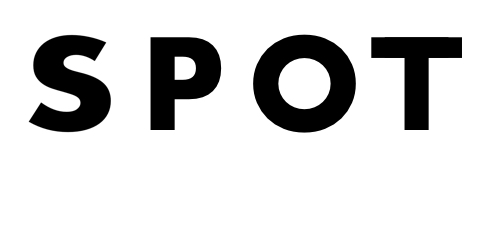
\includegraphics[width=0.6\linewidth]{spot.pdf}
        \caption{%
            Time evolution of a Gaussian absorption line on a rigidly rotating, spotted star computed from the analytic formulae in \S\ref{sec:kT}.
            The stellar surface is modeled as a spherical harmonic expansion up to $l_\mathrm{max}=20$, and the line shape is assumed to be the same everywhere;
            the spot simply downweights the local intensity at all wavelengths.
            As the spot rotates into view (left panel), the line shape changes slightly (center panel). 
            The residuals between the line when the spot is in view (solid) and when it is on the backside of the star (dotted) are shown in the right panel, where a Gaussian-like feature can be seen tracking the spot as it rotates from the blueshifted hemisphere to the redshifted hemisphere of the star.
        }
        \label{fig:spot}
    \end{centering}
\end{figure}

Figure~\ref{fig:compare} shows one of the spectra in Figure~\ref{fig:spot}, this time computed using both our formulae (blue line) and the traditional technique of discretizing the stellar surface, Doppler-shifting the spectrum in each grid cell according to the local radial velocity, interpolating back to a uniform wavelength grid, and summing over the spatial dimension (dotted orange line). 
We show the residuals in the lower panel, where it is clear that as the number of grid cells increases from 2,000 (light grey) to 71,000 (dark grey), the numerical solution approaches the solution obtained using our approach.

%Understand---and comment on---the fundamental
%differences between a discrete linear convolution and traditional linear 
%interpolation. Should we expect the numerical solution to actually \emph{converge}
%to the \starry solution, or is the way the two are interpolating fundamentally
%different?

\begin{figure}[t!]
    \begin{centering}
        \includegraphics[width=0.65\linewidth]{compare.pdf}
        \caption{%
            The observed spectrum when the spot is in view computed with
            \starry (blue) and numerically (orange). 
            The problem setup is the same as that in Figure~\ref{fig:spot}. 
            The bottom panel shows the absolute value of the difference between the two spectra for different number of grid points in the numerical solution.
            As the number of grid points increases, the numerical solution approaches the \starry solution.
        }
        \label{fig:compare}
    \end{centering}
\end{figure}

\end{document}